% \subsection{Command-Line Interface}
The compiled binary uses a command-line interface to configure and run one of many subcommands available.
These subcommands are:\label{sec:DesignSubcommands}
\begin{itemize}
    \item \texttt{makeinput}, which generates simulation input files, fulfilling \cref{req:GenerateState}.
    \item \texttt{fixedtime}, which runs a headless simulation for a fixed time, fulfilling \cref{req:HeadlessSim}.
    \item \texttt{compare}, which compares two simulation states for equality (see \cref{sec:Comparisons}), fulfilling \cref{req:Compare}.
    \item \texttt{renderppm}, which visualizes a static simulation state using the techniques from \cref{sec:Research:Viz:ACA}.
    % \item \texttt{convert2newbinary}, for converting ACA simulation state files to a potential new format (see \cref{sec:FileFormat}). Currently a no-op.
    \item \texttt{run}, which starts a real-time visualized simulation, fulfilling \cref{req:VizSim}.
\end{itemize}
Splitting the program into subcommands was inspired by Git\cite{tool:Git}, and avoids creating separate binaries for each operation.
Each subcommand can be configured with command-line options conforming to POSIX standard\cite{IEEE2018UtilityConventions}.
Examples of using the program are in \cref{fig:BashExampleUsage}.
\begin{figure}[ht]
    \centering
    \begin{lstlisting}[language=bash]
# Create an input file based on simple_layout with a size of 1x2 metres
./sim_cuda makeinput ./simple_layout.png 1 2 ./initial.bin

# Run it in headless mode for 10 seconds
./sim_cuda fixedtime --backend=cuda ./fluid.json ./initial.bin 10 \
                        -o ./output_after_10.bin

# Compare it to the expected output
./sim_cuda compare ./output_after_10.bin ./expected_after_10.bin

# Render it out to an image
./sim_cuda renderppm ./output_after_10.bin zeta ./output_after_10.ppm

# Try visualizing it in real-time
./sim_cuda run --backend=cuda ./fluid.json ./initial.bin
\end{lstlisting}
    \caption{Example usage of the simulation program}
    \label{fig:BashExampleUsage}
\end{figure}

\subsection{Generating Inputs}
The \texttt{makeinput} subcommand allows input simulation states to be generated from image files.
Each pixel of the input image represents a cell of the grid, including padding cells\footnote{This can allow the padding cells to be fluids rather than boundaries, which is incorrect. In the future this will be changed to add padding cells once the image is parsed.}, where non-black pixels are denoted as boundary cells and are fluid cells otherwise.
The example in \cref{fig:ExampleMakeinput} shows an example file which creates a rectangular obstacle, and the visualization of the generated state.
\begin{figure}[ht]
    \centering

    \subcaptionbox{Base Image%
    }[\linewidth]{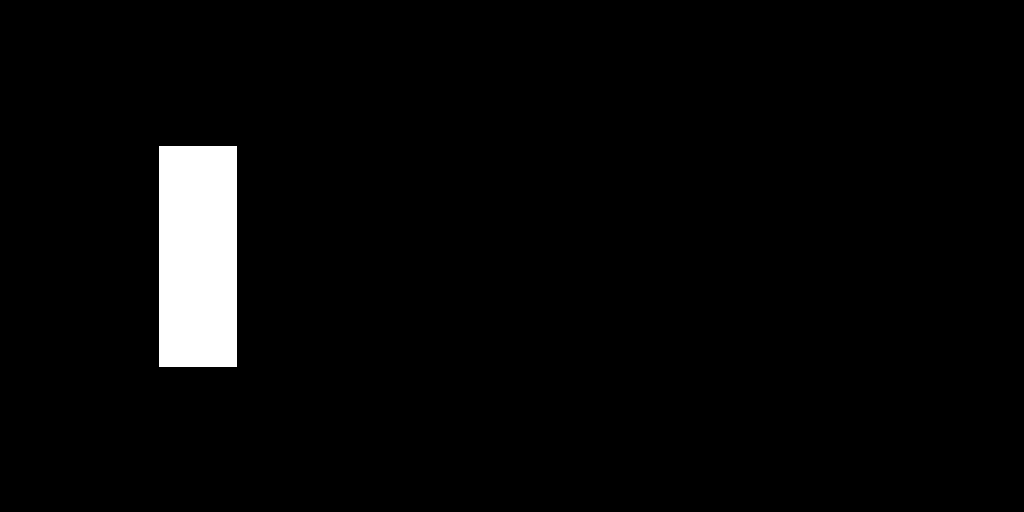
\includegraphics[]{Ch42Design/figures/simple_layout.png}
    }
    
    \subcaptionbox{Simulation%
    }[\linewidth]{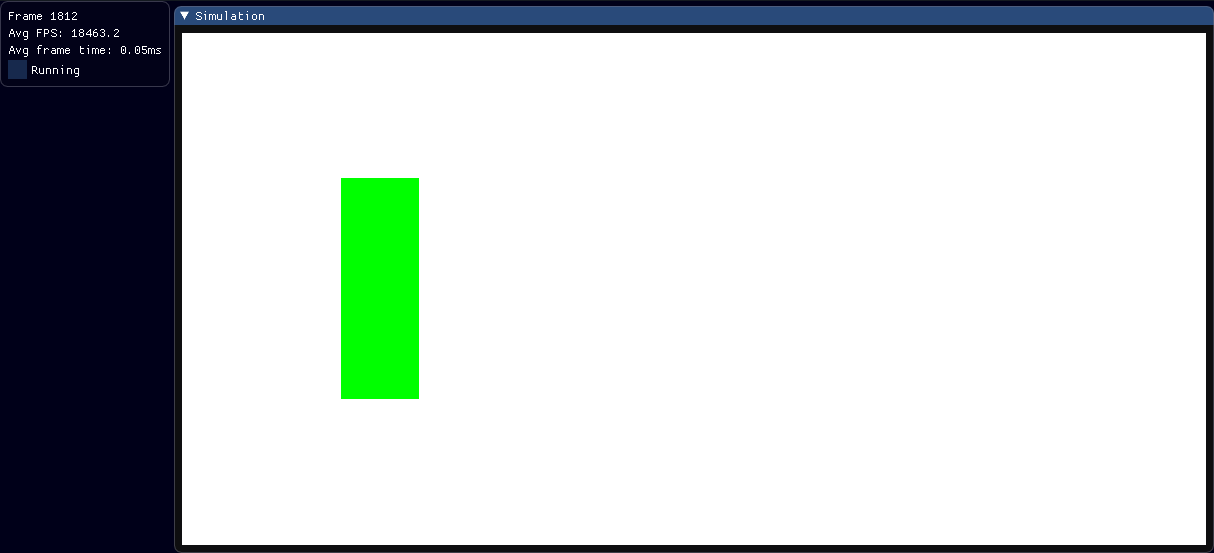
\includegraphics[width=0.5\linewidth]{Ch42Design/figures/example_sim_of_simple_layout.png}
    }
    
    \caption{Example conversion of an image to a simulation state}
    \label{fig:ExampleMakeinput}
\end{figure}

Velocities and pressure in every cell are interpolated horizontally - \SI{1}{m/s} east at the left edge, \SI{0}{m/s} at the right.
This alleviates simulation instability near obstacle edges, an advantage over having a constant initial velocity across the field.
% For velocities, this is \SI{1}{m/s} east, equal to the default flow of incoming fluid, which may cause issues with correctness.
One such instability would be a situation where fluid is occluded from the input direction by an obstacle, but moves east anyway with no reason to do so.
%it would not be correct for that fluid to move) 
% This will likely be changed to zero out initial velocity, requiring some simulation to take place before the fluid begins to move.

The exact initial value of pressure is inconsequential as the simulation only cares about the difference between cells.
The pressure is set to 0 at all points, representing a constant pressure across the simulation grid.
This is inconsistent with the nonzero velocities mentioned above, but applying variable pressure made the system more unstable.